% \chapter{Προεπεξεργασία \en{(Preprocessing)}}
% Στο κεφάλαιο αυτό  παρουσιάζεται αναλυτικά το στάδιο της Προεπεξεργασίας \en{(Preprocessing)}. Θα παρουσιαστούν εκτενώς όλες οι μέθοδοι και οι τεχνικές που χρησιμοποιήθηκαν, ο σκοπός τους και η τελική μορφή των δεδομένων. 

% Είναι σημαντικό να γίνει κατανοητή η σημαντικότητα αυτού του σταδίου για την ακρίβεια των τελικών αποτελεσμάτων. Το αρχικό μας σύνολο δεδομένων περιέχει δύο είδη πληροφορίας. Τη χρήσιμη για τον ερευνητικό σκοπό και όλη την υπόλοιπη η οποία, εάν δεν απομονωθεί σωστά, ενδέχεται να προκαλέσει αλλοίωση των αποτελεσμάτων, εκπαίδευση του συστήματος προς λανθασμένη κατεύθυνση και σίγουρα ανώφελη κατανάλωση υπολογιστικής ισχύος αλλά και χρόνου.

% Σε αυτό το στάδιο ο ερευνητής πρέπει να παρατηρήσει σωστά την πληροφορία και να κρατήσει το ωφέλιμο κομμάτι με σκοπό να έχει πιο ποιοτικά δεδομένα, προσέχοντας στην προσπάθεια αυτήν να μην απωλέσει κομμάτι χρήσιμης πληροφορίας που θα εκπαίδευε σωστά το σύστημα.


% \section{Βήμα 1: Μείωση κατηγοριών και απομόνωση πεδίων}
% Είδαμε οτι στο συγκεκριμένο \en{dataset} υπάρχει μεγάλη ανομοιομορφία ως προς την κατανομή των δεδομένων στις διάφορες κατηγορίες. Αυτό αποτελεί ένα μείζον πρόβλημα στους αναλυτές δεδομένων, γνωστό ως \en{Imbalanced Data}, το οποίο οδήγησε την κοινότητα στην ανάπτυξη διάφορων τεχνικών αντιμετώπισης του. Το μεγαλύτερο πρόβλημα έγκειται στο ότι οι αλγόριθμοι ταξινόμησης υποθέτουν οτι όλες οι κλάσεις έχουν ίδο πλήθος δεδομένων και εκπαιδεύονται εξ'ίσου σε όλες.

% Επομένως, στο πρώτο βήμα, εξαλείφουμε τις μειονότητες με σκοπό να οδηγηθούμε σε ένα κάπως πιο ισορροπημένο σύνολο δεδομένων. Πρατικά, φιλτράρουμε τα δεδομένα έτσι ώστε να εξαλειφθούν οι κατηγορίες που έχουν λιγότερα απο 50 στοιχεία. 

% Εμφανίζουμε ξανά το πλήθος των κατηγοριών και των εγγραφών ανά κατηγορία, καθώς και τη γραφική απεικόνιση σε διάγραμμα μέσω της βιβλιοθήκης \en{matplotlib}. Τα αποτελέσματα φαίνονται στα Σχήματα ~\ref{figure4.1} και ~\ref{figure4.2}
% \clearpage

% \begin{figure}\centering
% 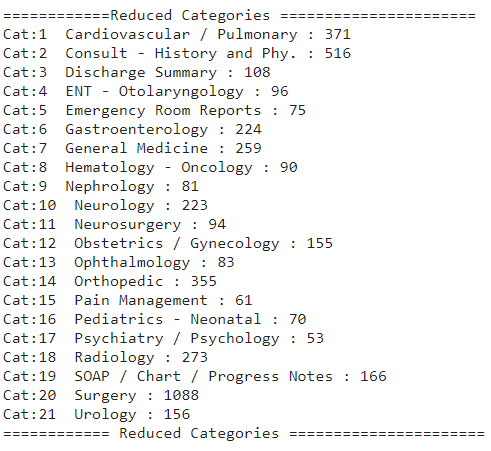
\includegraphics[width=\textwidth,height=9cm,keepaspectratio]{pictures/3reducedCategories.png} \caption{Το πλήθος εγγραφών ανά κατηγορία μετά την εξάλειψη των μειονοτήτων.}\label{figure4.1}
% \end{figure}

% \begin{figure}\centering
% 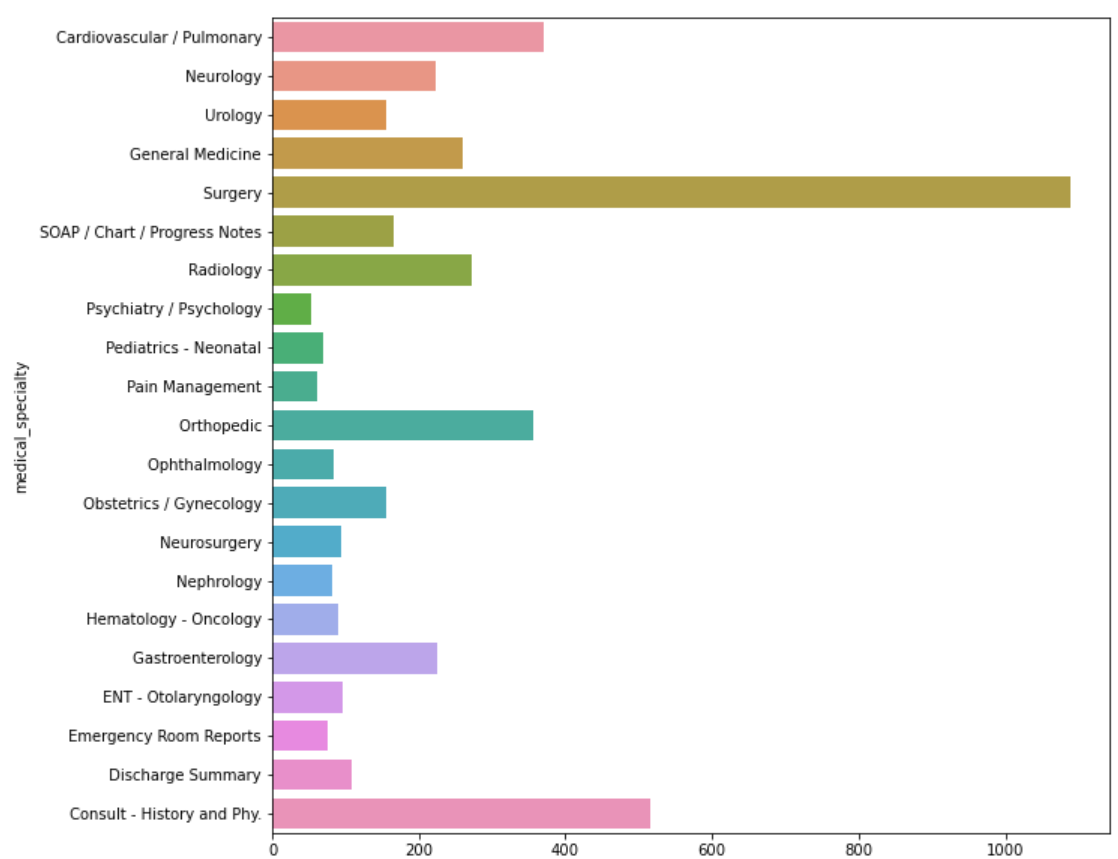
\includegraphics[width=\textwidth,height=14cm,keepaspectratio]{pictures/3categoriesPlot.png} \caption{Γραφικη απεικόνιση του σχήματος 4.1}\label{figure4.2}
% \end{figure}
% \clearpage
% Είδαμε ότι το σύνολο των δεδομένων αποτελείται απο έξι πεδία εκ των οποίων μας αφορούν μόνο δύο:

% 1) Το πεδίο \en{medical\_specialty} το οποίο αναφέρεται στην κατηγορία/ειδικότητα στην οποία έγκειται το περιστατικό και 

% 2) Το πεδίο \en{transcription} το οποίο είναι το κυρίως κείμενο και αναφέρεται στην περιγραφή του περιστατικού.  

% Επομένως τα δεδομένα φιλτράρoνται ξανά με σκοπό να κρατηθεί μόνο η πληροφορία αυτών των δύο πεδίων και στη συνέχεια αποθηκεύονται σε έναν πίνακα, εμφανίζοντας στο τέλος το πλήθος στηλών και γραμμών. 

% Τα δεδομένα πλέον έχουν την εξής μορφή : \en{[4597 rows x 2 columns]}

% \section{Βήμα 2: Kαθαρισμός κειμένου (\en{text cleaning})}

% Στη συνέχεια εκτελείται η διαδικασία καθαρισμού κειμένου (\en{text cleaning process.}) Αρχικά ορίζονται δύο συναρτήσεις: η \en{clean\_text()} και η \en{lemmatize\_text()} οι οποίες επιτελούν τις παρακάτω διεργασίες: 
% \begin{enumerate}
%     \item Διαίρεση σε όρους \en{(Tokenization)}:
%     Με αυτόν τον όρο αναφερόμαστε τον κατακερματισμό μιας συμβολοσειράς σε διακριτές λέξεις. Ο κάθε όρος μπορεί να είναι ολόκληρη λέξη, μεμονομένος χαρακτήρας, αριθμός, σύμβολο ή σημείο στίξης. \cite{lemmatize}. Σε αυτήν την εργασία, η κάθε εγγραφή του πεδίου \en{transcription}, που αποτελούν το κείμενο προς επεξεργασία, χωρίζεται σε λέξεις. Η μορφή των δεδομένων τώρα είναι ένας πίνακας όπου το κείμενο παρουσιάζεται σε μορφή λίστας με διακριτούς όρους.
    
%     \item Αφαίρεση λέξεων χωρίς νοηματική αξία \en{stopwords removal}:
%     Ένα από τα πιο συνηθισμένα βήματα προεπεξεργασίας κειμένου φυσικής γλώσσας είναι η αφαίρεση λέξεων χωρίς ιδιαίτερη νοηματική αξία. Η βιβλιοθήκη \en{NLTK} της \en{Python} προσφέρει αυτή τη δυνατότητα, απομακρύνοντας λέξεις που δεν αποδίδουν χρήσιμη πληροφορία, αντιθέτως προσθέτουν στο κείμενο θόρυβο και όγκο. Αυτό γίνεται είτε μέσω έτοιμης λίστας \en{stopwords}, είτε εντοπίζοντας λέξεις που εμφανίζονται εξαιρετικά συχνά σε ένα κείμενο. Τέτοιες λέξεις μπορεί να είναι άρθρα, αντωνυμίες, ακόμα και πολύ συνηθισμένα ρήματα.
    
%     \item Μετατροπή κεφαλαίων χαρακτήρων σε πεζούς:
%     Εδώ γίνεται χρήση της μεθόδου \en{.lower()} που προσφέρει η  \en{python} για μετατροπή συμβολοσειρών, η οποία μετατρέπει οποιοδήποτε κεφαλαίο χαρακτήρα σε πεζό.
    
%     \item Απομάκρυνση αριθμών και συμβόλων:
%     Οι αριθμοί, τα σύμβολα και τα σημεία στίξης, για το σκοπό της εργασίας, αποτελούν περιττή πληροφορία. Απαλάσσοντας το κείμενο από αυτά μειώνεται ο όγκος εργασίας, η απαιτούμενη υπολογιστική ισχύς και παράγονται πιο ποιοτικά δεδομένα. Έτσι με χρήση κατάλληλων εντολών της \en{python}, όλα αυτά αφαιρούνται.
    
%     \item \en{Stemming}
%     Ο όρος \en{Stemming} αναφέρεται σε μια διαδικασία που παρέχεται απο τη βιβλιοθήκη \en{NLTK} της \en{Python} η οποία ανάγει όλες τις ομόρριζες λέξεις του κειμένου στην αρχική τους ρίζα, αδιαφορώντας για τις διαφορετικές καταλήξεις που ενδεχομένως να έχουν. Για παράδειγμα, η λέξη \en{coding} ανάγεται στη λέξη \en{code}.
    
%     \item Λημματοποίηση \en{(Lemmatization)}
%     Ο όρος λημματοποίηση αναφέρεται στη διαδικασία επεξεργασίας κειμένου φυσικής γλώσσας με σκοπό να φέρει την κάθε λέξη σε μια μορφή τέτοια, ώστε να υπάρχει όσο το δυνατόν μικρότερη ποικιλία στο συνολικό λεξιλόγιο, επιδιώκοντας την επιστροφή των λέξεων στο αρχικό τους λήμμα. Η βασική διαφορά των δύο τελευταίων διαδικασιών ειναι οτι στη λημματοποίηση εξετάζεται η γλωσσολογική προέλευση κάθε όρου ώστε να βρεθεί το κατάλληλο λήμμα. Αποτελεί μια πιο εξελιγμένη διαδικασία καθώς το \en{stemming} δεν εξετάζει πληροφορίες που αφορούν τη γλωσσολογική προέλευση της λέξης, αλλά μόνο τη σχέση ρίζας - κατάληξης. Χρησιμοποιώντας και πάλι τη βιβλιοθήκη \en{NLTK} της \en{Python}, γίνεται ομαδοποίηση των λημμάτων μέσω της μεθόδου \en{WordNetLemmatizer()} με βάση το λεξικό \en{WordNet} Για παράδειγμα, στο \en{lemmatization}, η λέξη \en{better} ανάγεται στη λέξη \en{good}.
% \end{enumerate}

% Σε αυτό το σημείο, η λίστα κειμένων είναι απαλλαγμένη από στοιχεία που προσδίδουν αχρείαστο όγκο, θόρυβο και περιττή πληροφορία. Στα επόμενα κεφάλαια θα χρησιμοποιηθεί το σύνολο δεδομένων με το "καθαρισμένο" κείμενο ως είσοδο στα προγράμματα με σκοπό την εκπαίδευση του συστήματος και την παραγωγή γνώσης.